\documentclass[sigchi-a]{acmart}
\usepackage{booktabs} % For formal tables
\usepackage{ccicons}  % For Creative Commons citation icons

\begin{document}
\fancyhead{}
% Copyright
\copyrightyear{2019} 
\acmYear{2019} 
\setcopyright{acmcopyright}
\acmConference[CHI'19 Extended Abstracts] {CHI Conference on Human Factors in Computing Systems Extended Abstracts}{May 4--9, 2019}{Glasgow, Scotland UK}
% Note UK should be in caps
\acmBooktitle{CHI Conference on Human Factors in Computing Systems Extended Abstracts (CHI'19 Extended Abstracts), May 4--9, 2019, Glasgow, Scotland UK}
\acmPrice{}
\acmISBN{978-1-4503-5971-9/19/05}
\acmDOI{10.1145/3290607.3312761}
% Authors, replace the red X's with your assigned DOI string during the rightsreview eform process.

\settopmatter{printacmref=true}

%\acmBadgeL[http://ctuning.org/ae/ppopp2016.html]{ae-logo}
%\acmBadgeR[http://ctuning.org/ae/ppopp2016.html]{ae-logo}


%\title{Explore the Configuration for Augmented Communication}
%\title {Exploring Placement of Users and Content for Augmented Communication in Mixed Reality}
\title {Exploring Configuration of Mixed Reality Spaces for Communication}

\author{Zhenyi He}
\affiliation{%
  \institution{New York University}
  \city{New York}
  \state{NY}
  \postcode{10011}
  \country{USA} }
\email{zh719@nyu.edu}

\author{Karl Toby Rosenberg}
\affiliation{%
  \institution{New York University}
  \city{New York}
  \state{NY}
  \postcode{10011}
  \country{USA} }
\email{ktr254@nyu.edu}

\author{Ken Perlin}
\affiliation{%
  \institution{New York University}
  \city{New York} \postcode{10011} \country{USA}}
\email{ken.perlin@gmail.com}

\settopmatter{printacmref=false}
% The default list of authors is too long for headers.
%\renewcommand{\shortauthors}{F. Author et al.}

%
% The code below should be generated by the tool at
% http://dl.acm.org/ccs.cfm
% Please copy and paste the code instead of the example below.
%

%\newcommand{\zhenyi}[1]{{\color{red} #1}}
%\newcommand{\red}[1]{\textcolor{red}{#1}}

\ccsdesc[500]{Human-centered computing~Mixed / augmented reality}
\ccsdesc[300]{Human-centered computing~Collaborative interaction}


\newcommand{\zhenyi}[1]{{\color{black} #1}}
\newcommand{\karl}[1]{{\color{black} #1}}
\definecolor{armygreen}{rgb}{0.29, 0.53, 0.13}
\newcommand{\karlZhenyiEdits}[1]{{\color{black} #1}}



\begin{abstract}
  %Abstracts should be about 150 words. Required.
  
  \karlZhenyiEdits {
  Mixed Reality (MR) enables users to explore scenarios not realizable in the physical world. This allows users to communicate with the help of digital content. We investigate how different configurations of participants and content affect communication in a shared immersive environment. We designed and implemented side-by-side, mirrored face-to-face and eyes-free configurations in our multi-user MR environment and conducted a preliminary user study for our mirrored face-to-face configuration, evaluating with respect to one-to-one interaction, smooth focus shifts and eye contact within a 3D presentation using the interactive Chalktalk system. We provide experimental results and interview responses.
  }
  
\end{abstract}


%\keywords{immersive learning; mixed reality}

\begin{marginfigure}
    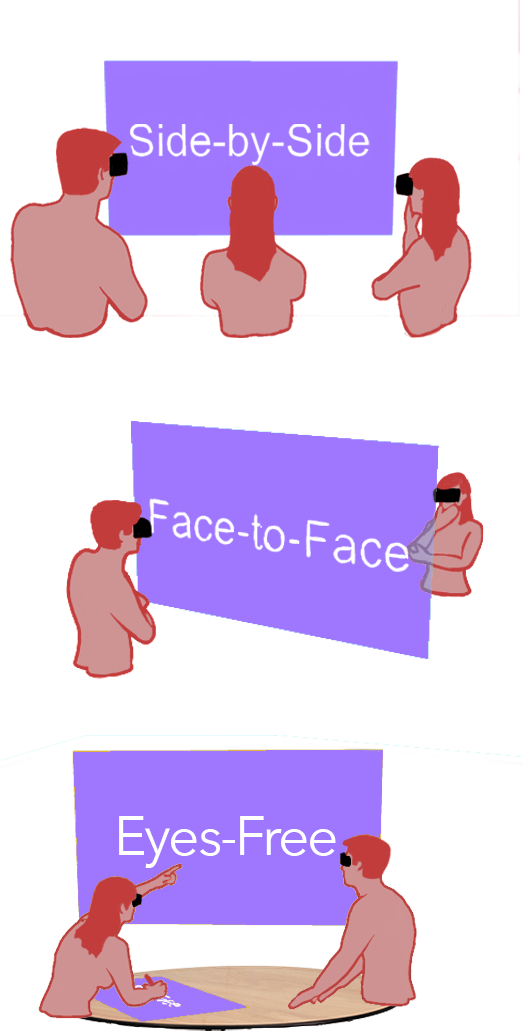
\includegraphics[width=\marginparwidth]{configurations}
    \caption{Three Configurations for MR Communication. \\Inspiration for configurations:
1) side-by-side whiteboard brainstorming, 
2) daily face-to-face conversations and
3) drafting boards}

    \label{fig:config}
\end{marginfigure}


\begin{margintable}
\vspace{1cm}
\flushleft
\textbf{KEYWORDS}\\
Mixed reality; communication; collaboration;
\end{margintable}
\maketitle


%\begin{figure}
%  
\includegraphics[width=\marginparwidth]{sigchi-logo}\Description{SIGCHI
%    logo} 
%  \caption{Insert a caption below each figure.}
%  \label{fig:sample}
%\end{figure}



\section{Introduction}
\begin{margintable}
    \caption{Terminology Table}
    \label{tab:table1}
    \begin{tabular}{p{1.6cm} p{3.81cm}}
      \textbf{Term} &  \textbf{Definition}
      \\
      \toprule
      Content Creation Server & The content creation server is an external server which takes raw drawing point data as the input, recognizes the drawing, and creates interactive objects. \\
      Content Board & The content board is the transparent area on which content is displayed.
      The user's input will be projected to the content board and sent to the content creation server for processing. Afterwards, the result will be displayed in 3D in the transparent area.
      \\
      Configuration & The configuration refers to the placement and orientation of users and the content board with respect to each other. \\
      \bottomrule
    \end{tabular}
\end{margintable}

Virtual Reality and Mixed Reality (VR, MR) are being explored increasingly, spurred by the availability of high quality consumer headsets in recent years. VR and MR enable rich design spaces in HCI by providing 3D input and immersive experiences. Decades ago, the "Office of the future" was proposed to allow remotely located people to feel as though they were together in a shared office space~\cite{raskar1998office}, via a hybrid of modalities including telepresence, large panoramic displays and shared manipulation of 3D objects. The core idea was that VR/MR had the potential to enhance communication among groups of people. Since then, significant progress has been made in exploring techniques for communication ~\cite{ishii1993integration, otsuka2016mmspace}. However, less studied is the configuration (see our full definition in table~\ref{tab:table1}) of people and shared manipulable objects in the environment, which may lead to different communication experiences.

In daily life while speaking to others, we commonly use gestures or visual aids to help present ideas, either subconsciously or purposefully. Visual aids can be drawn on paper, a whiteboard, or a screen via video chat. A key task for collaborators is the shifting of focus between spoken words, gestures and visual aids such as notes and drawings. Smooth transitions in conversations have been found to be important for collaboration~\cite{buxton1992telepresence}.
Prior work addressed this with alternative configurations of spaces for communication. Tan et al. built a face-to-face presentation system for remote audiences ~\cite{gazeAwareness}. ClearBoard~\cite{ishii1993integration} created a shared workspace in which two users collaborate remotely without losing all the advantages of in-person face-to-face interactions. One such advantage relates to learning. When a teacher looks away from the audience, Lanir et al. ~\cite{Lanir2008ClassroomPresentationSoftware} observed that audiences in a classroom would not focus on the presenter, which might "create a learning environment in which there is no interpersonal engagement between the presenter and the audience, thus reducing learning outcomes." 
We find that personal engagement, such as one-to-one interaction and eye contact~\cite{InsaPositionInClassroom}, in addition to focus shift~\cite{buxton1992telepresence}, is therefore relevant to evaluating communication experiences.

Still, it is unclear how the configuration of users and content in an MR space affects communication for co-located and distant people.
We have implemented a multi-user MR workstation to explore how configuration impacts communication by providing three different configurations: 1) side-by-side, 2) mirrored face-to-face and 3) eyes-free. We conducted a preliminary user-study of the mirrored face-to-face configuration.
Afterwards, we proceeded to user interviews in which participants spoke about the face-to-face experience, one-to-one interaction, focus shift and eye contact. %And describe plans for future research, which include user-studies for each configuration, as well as comparing the configurations.

\section{Related Work}
Much work has been done in collaborative applications in VR/MR. T(ether) is a spatially-aware display system for co-located collaborative manipulation and animation of objects ~\cite{lakatos2014t}. Trackable markers on pads and digital gloves allow participants to use gestures to manipulate objects in space. Virtual Replicas for Remote Assistance is a remote collaboration system, allowing a remote expert to guide local users to assemble machine parts by using virtual replicas~\cite{oda2015virtual}.
SpaceTime is a scene editing tool supporting multi-user collaboration in VR, either co-located or remote~\cite{xia2018spacetime}. To support conflict resolution when two users wish to work on the same object simultaneously, SpaceTime creates per-user branches of the object, which can later be merged. 
Rather than enhancing experiences for specific tasks, our system aims to enhance the experience of general communication, which can benefit various kinds of more specific collaborative work.

%TODO bolden the outline for content creation server
\begin{marginfigure}
    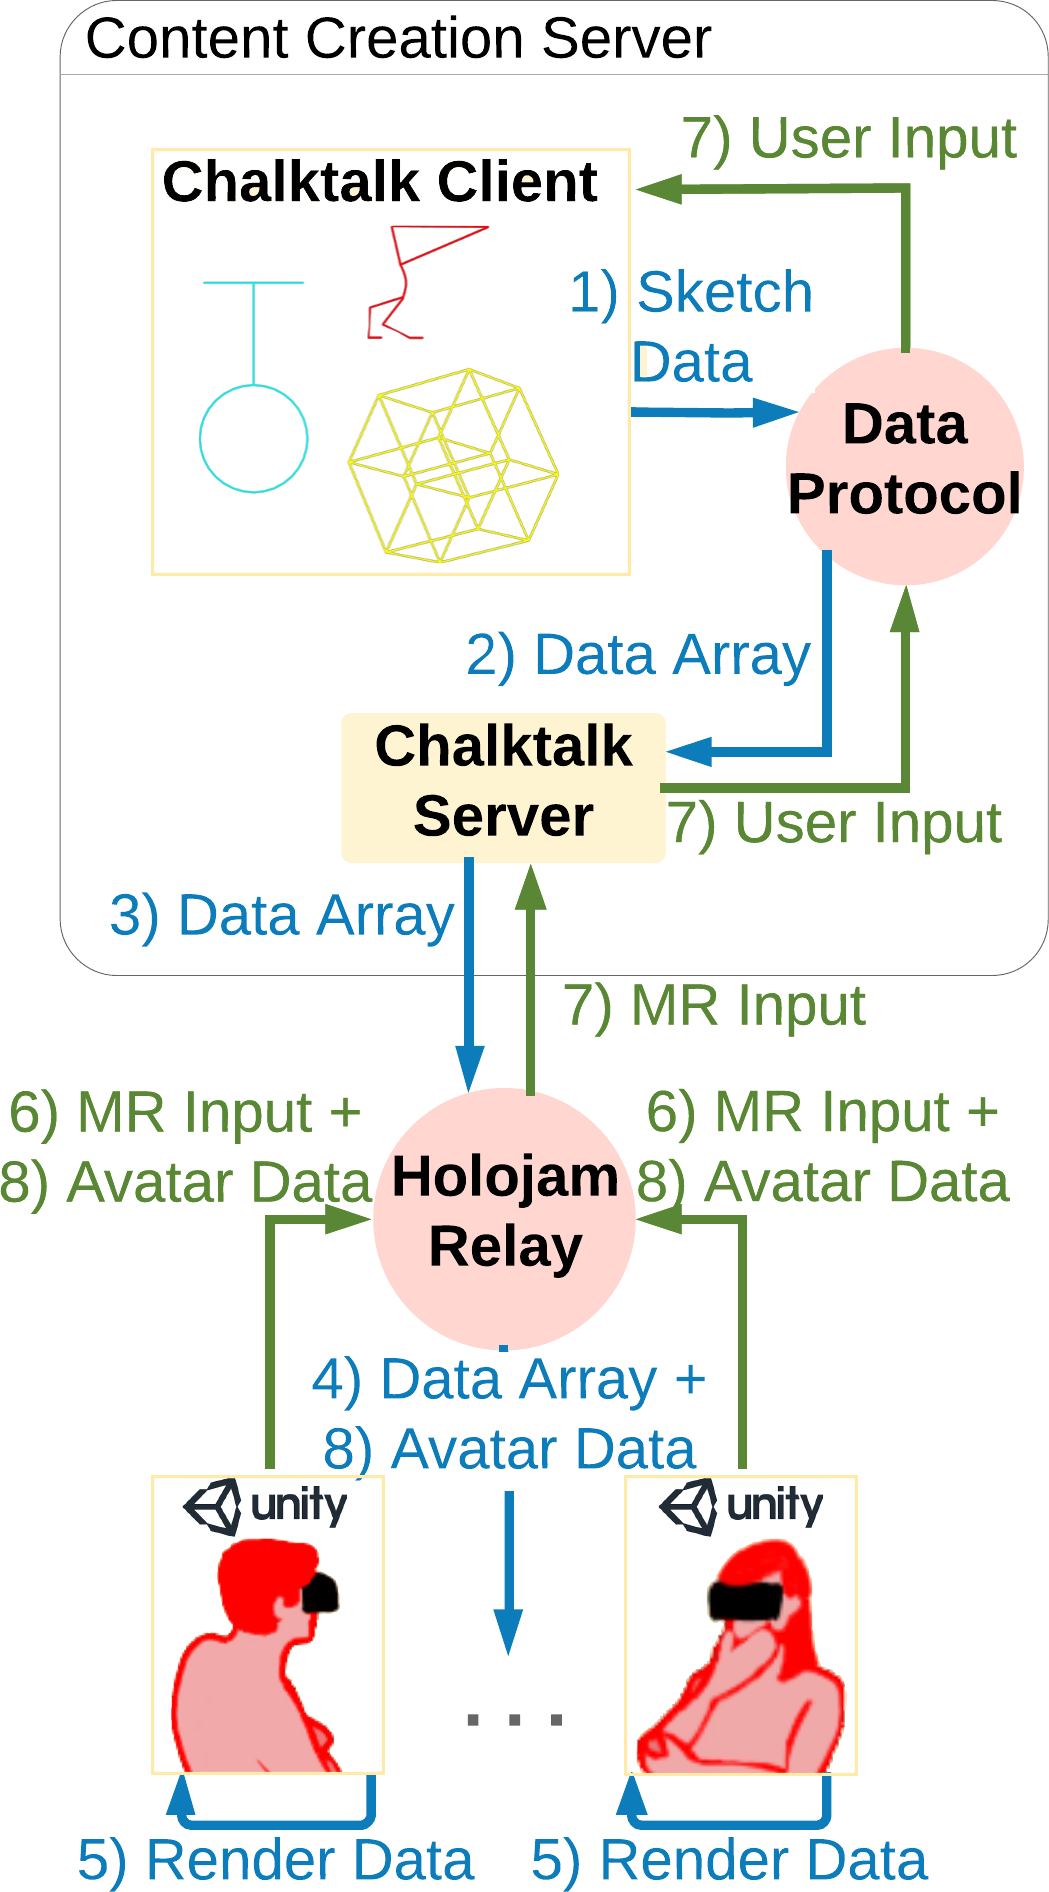
\includegraphics[width=0.85\marginparwidth]{dataflow2}
    \caption{Data Pipeline}
    \label{fig:datapipeline}
\end{marginfigure}
\begin{sidebar}
%   Chalktalk's content ("sketches") is is composed of graphical elements such as point data. In the Chalktalk client we serialize all sketch data(1) into a data array(2), which is sent to the Chalktalk server, then (3) to the Holojam relay. The Holojam relay multicasts the data array(4) to all Unity clients. The clients de-serialize and parse the array into render data(5) that are displayed on MR content board(s). MR user input data(6) on the Unity client-side is also transformed and sent back through the Holojam relay and Chalktalk server to the Chalktalk client. The Chalktalk client then translates the input data(7) into HTML canvas mouse events that it understands. Unity clients can see each other correctly by synchronizing avatar data(8).
 
 
 Chalktalk's content ("sketches") is composed of graphical elements such as point data. 1) Sketch data are serialized on the Chalktalk client side every frame and 2) sent as a data array to the Chalktalk server, 3) to the Holojam relay, and then 4) to all Unity clients, where 5) the data are rendered on content board(s). 6) MR user input is sent back through the pipeline to the Chalktalk client and 7) translated into HTML canvas mouse events. 8) Avatar synchronization data are also sent between clients using the Holojam relay.
 
  
  %Users can control Chalktalk from within the MR environment without needing Chalktalk to know the specifics of Unity or of the VR device. 
  %Due to the use of this generic protocol, users are able to generate and interact with Chalktalk content without requiring a re-implementation of Chalktalk in Unity.
  %\caption{Data Pipeline}
  %\label{bar:sidebar}
\end{sidebar}

Some previous work contributed to communication in VR/MR too. ClearBoard allows a pair of users to shift easily between interpersonal space and a shared workspace~\cite{ishii1993integration}.
The key metaphor of ClearBoard is ``talking through and drawing on a big transparent glass board.'' No gaze or eye contact information is lost while working on the content. ShareVR enables communication between an HMD user and a non-HMD user~\cite{gugenheimer2017sharevr}. By using floor projection and mobile displays to visualize the virtual world, the non-HMD user is able to interact with the HMD user and become part of the VR experience. The work discusses how people with different devices communicate with each other. MMSpace allows face-to-face social interactions and telepresence in the context of small group remote conferences~\cite{otsuka2016mmspace}. It uses custom-built mechanical displays on which images of remote participants are projected, and which move in response to users' movements. Pairs of participants can maintain eye contact with each other and remain aware of each other's focus. Instead of designing a configuration to fit one specific communication use case, we provide three different configurations for general-purpose communication in VR/MR.


\section{Detailed design and implementation}

\textit{Three Configuration Designs.}
We implemented three \textit{configurations} for communication in our system: 1) side-by-side, 2) mirrored face-to-face and 3) eyes-free (see figure~\ref{fig:config}).
For 1), our implementation has users facing a \textit{content board} (see full definition in table~\ref{tab:table1}) from the same side.

% For 2), the users are face-to-face in the virtual environment with the content board placed between them, so that each sees the other on the opposite side of the content board, left-right reversed as if reflected in a mirror. Mirror reversal allows, for example, text to be readable for both participants.
% %and asymmetric objects will appear differently on one side. 
% The challenge is ensuring all the content is consistent
% %and legible 
% for everyone on each side of the board.


%revised order
For 2), the users are face-to-face in the virtual environment with the content board placed between them, so that each sees the other on the opposite side of the content board, left-right reversed as if reflected in a mirror.
%and asymmetric objects will appear differently on one side. 
The challenge is ensuring all the content is consistent
%and legible 
for everyone on each side of the board. Mirror reversal allows, for example, text to be readable and asymmetric objects to appear correct for each participant.
ClearBoard~\cite{ishii1993integration} implemented "mirror reversal" via video capture and projection techniques to solve a similar problem for 2D displays. Inspired by that, we implemented a 3D immersive mirror reversal for our MR configuration. We place the users physically
%(in the real world)
on the same side of the content board and mirror all other users (from one user's perspective) to the other side. This way, information such as gaze and gesture direction is preserved, so participants can know where each other is looking and pointing (see figure~\ref{fig:marginfig:mirror}).
%: person A is drawing a coordinate system with his right hand on the left side of the content board from his perspective, whereas person B sees person A drawing with the left hand. The content of the drawing appears the same way to both of them.

\begin{marginfigure}
    %\begin{subfigure}
        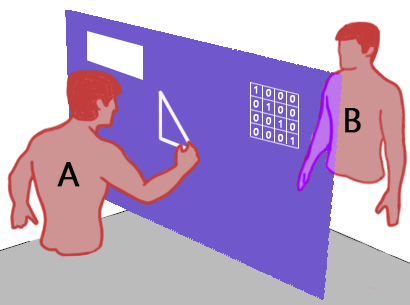
\includegraphics[width=0.75\marginparwidth]{personA}\\
        a. Person A's view. 
        %\label{fig:marginfig:mirror1}
        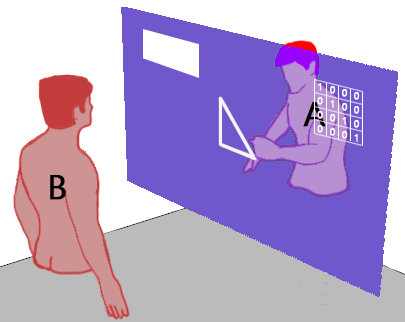
\includegraphics[width=0.75\marginparwidth]{personB}\\
        b. Person B's view.
        %\label{fig:marginfig:mirror2}
    %\end{subfigure}
    \caption{Mirrored Face-to-face Configuration Implementation. Person A is drawing a triangle with right hand from his perspective, whereas person B sees person A drawing with the left hand. The content of the drawing appears the same to both.}
    \label{fig:marginfig:mirror}
\end{marginfigure}

For 3), instead of writing or drawing in mid-air, users can create content in MR
%by writing 
while resting their arms atop a horizontal surface in the real world (e.g. table), thereby avoiding the potential fatigue of drawing in mid-air for long periods of time. For this configuration, we now have two boards in the MR world: a horizontal drafting board used for writing and drawing, and a vertical board that displays all information to be seen by all people in a group. All content is duplicated onto the vertical board. A cursor on the vertical board corresponds to the position of the user's hand on the horizontal board. This way, the person using the horizontal board need not look downward, remaining free to look at the vertical content board and other people. This allows users to pay more attention to the environment and each other in a shared experience. The configuration can extend 1) and 2) since we can choose where to place the vertical duplicate board.

\textit{The MR System.} Our system comprises 1) a content creation server, 2) an internal network framework and 3) VR/MR clients (see figure~\ref{fig:datapipeline} for a detailed description). 1) To enable interactive content during communication, we chose Chalktalk as our content creation server (see figure~\ref{fig:expMatrix}). Chalktalk is a web browser-based 3D presentation and communication tool
%written in JavaScript, 
in which the user draws interactive "sketches" for presentation. We designed a generic data serialization protocol to connect and decouple the content creation server and the VR/MR clients, so alternative content could easily be plugged in.
%to the system. 
2) To ensure communication between different devices, we used Holojam~\cite{perlin2016future}, a shared space network framework designed at our lab.
%and written in Node.js and C\#. 
It synchronizes data across devices and supports custom data formats.
%, so we can use our protocol. 
3) We implemented the VR/MR clients with Unity to support multiple VR/MR devices.


\section{Preliminary Experiment}

\begin{marginfigure}
    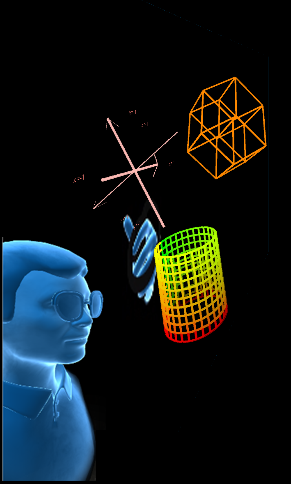
\includegraphics[height = 2.5cm]{3d.png}
    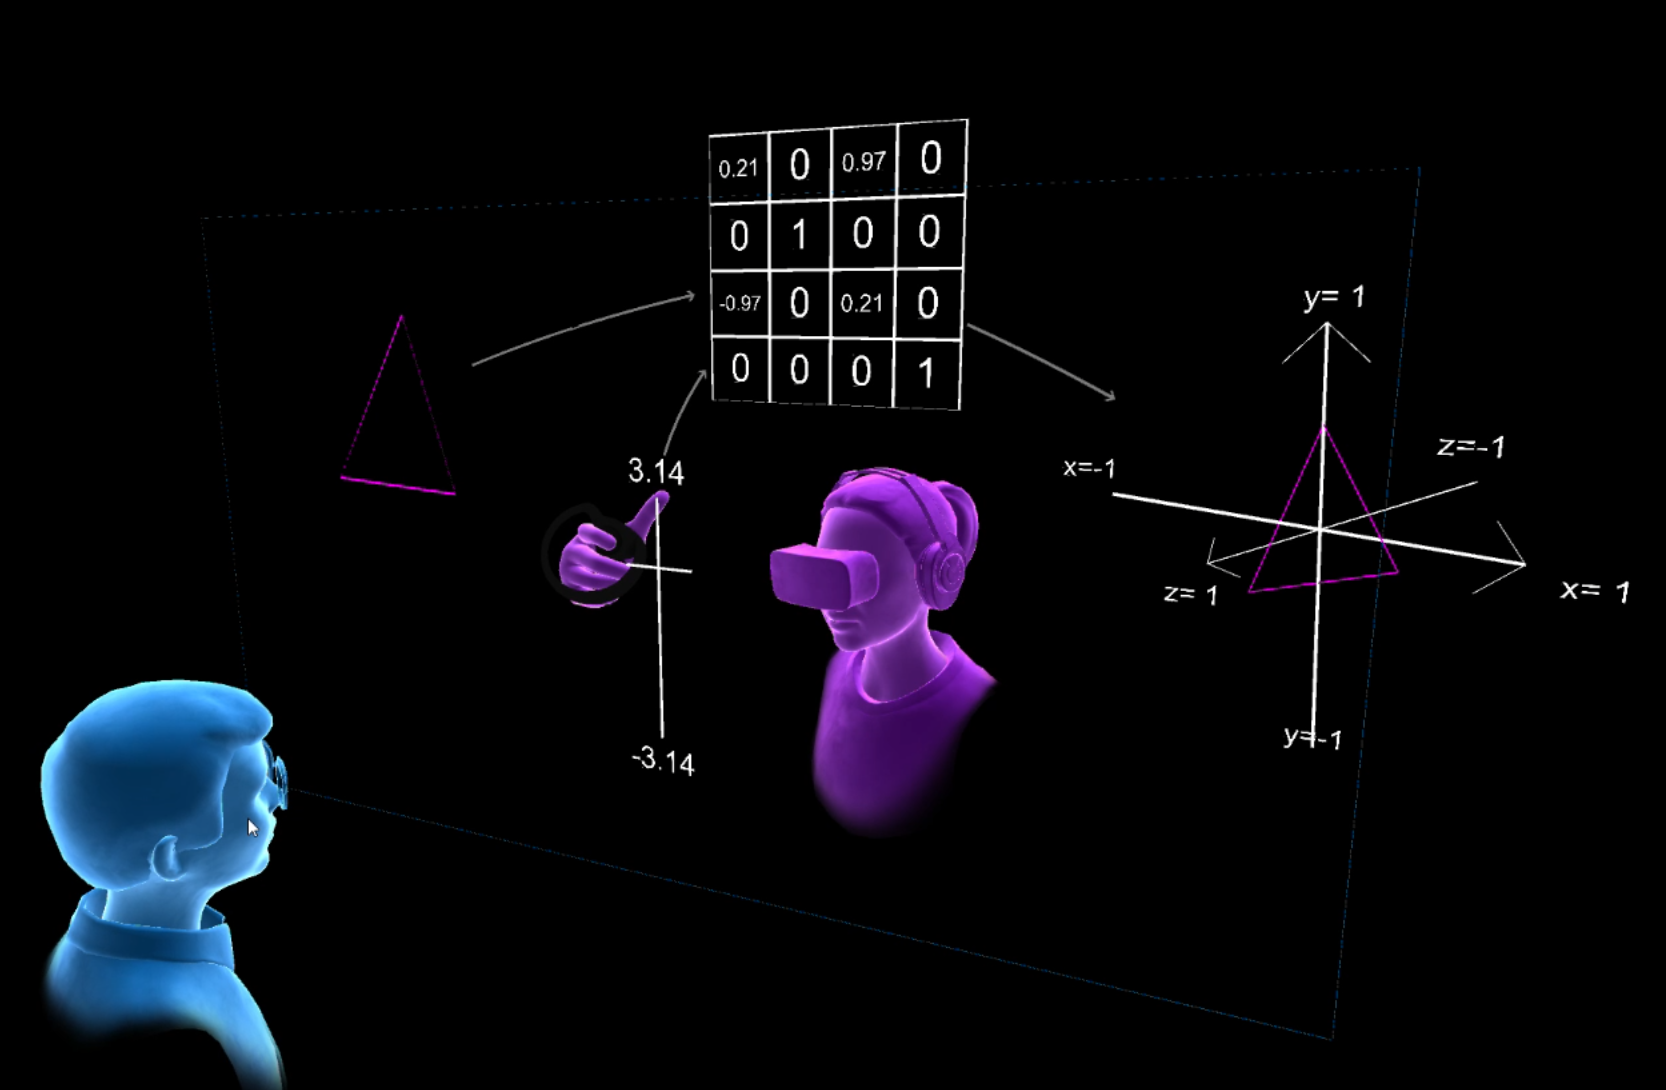
\includegraphics[height = 2.5cm]{experimentMatrix.png}
    \caption{Left: The content board is 3D. Right: Screenshot from experiment with matrix presentation.}
    \label{fig:expMatrix}
\end{marginfigure}

We plan to conduct experiments for each configuration design and to compare the configurations. So far, we have completed a preliminary user study on our mirrored face-to-face configuration, conducted with 8 participants (F=4) between the ages of 22 and 26 (M=23.71, SD=1.50), recruited via email and word-of-mouth.
%, including undergraduate and graduate computer science and art students from New York University studying either Computer Science or Art and Design. 
Participants were required to have taken a linear algebra class and to have prior experience with VR/MR. First, we introduced Chalktalk to participants who were unfamiliar with it to reduce the novelty effect. Then we gave a presentation on matrix transformations (a concept in the computer graphics curriculum, see figure~\ref{fig:expMatrix} and sidebar ~\ref{sidebar:matrix}) using our system in the mirrored face-to-face configuration. For each session, we had 1 presenter and 2 study participants in the audience, all physically remote. The presentation was repeated 4 times for 8 participants in all.
%\karl{To create a realistic presentation, we invited a computer graphics professor to present a lesson on matrices, and he permitted us to use his presentation as the basis for our experiment (see the rationale for our choice in topic and the steps in the presentation in sidebar ~\ref{sidebar:matrix}). }
We ran the experience with Oculus Rift headsets. Upon completion of all sessions, participants answered a questionnaire that gauged their opinions on one-to-one interaction~\cite{Lanir2008ClassroomPresentationSoftware}, eye contact~\cite{InsaPositionInClassroom} and focus shift~\cite{buxton1992telepresence} during the experience. Participants then joined a semi-structured exit interview. All factors were evaluated using the 7-point Likert scale. The study was recorded with users' permission.

% We chose the topic of matrix transformations so participants could see and interact with 3D moving content. For content within the 3D immersive environment, we chose visualization of the way a matrix translates and rotates geometry. To create a realistic presentation, we invited a computer graphics professor at our university to present on the subject (see detailed steps in sidebar~\ref{sidebar:matrix}), and he permitted us to use a recording of this sample presentation as the basis for our experiment. During the experiment, the presenter also made gestures and moved content around the MR space.

\begin{sidebar}
To create a realistic presentation, we invited a computer graphics professor to present a lesson on matrices. He permitted us to use his presentation as the basis for our experiment.
We chose the topic of matrix transformations so participants could see and interact with 3D moving content. 
For content within the 3D immersive environment, we chose visualization of the way a matrix translates and rotates geometry. 
%To create a realistic presentation, we invited a computer graphics professor at our university to present on the subject, and he permitted us to use a recording of this sample presentation as the basis for our experiment. During the experiment, the presenter also made gestures and moved content around the MR space.
During the lecture the presenter demonstrated matrix transformations, including translation and rotation, by using 3D interactive visualizations from the content server. Then she showed that matrix operations are non-commutative.
The following lists the steps in the presentation:
\begin{enumerate}
  \item The presenter creates a 4x4 rotation matrix object and links geometry to it. 
  \item Modifying the matrix values rotates the geometry in 3D space. Students are invited to walk around the MR environment to observe from any angle. 
  \item The presenter creates a second 4x4 matrix for translation, which she composes with the rotation matrix.
  \item To demonstrate that matrices are non-commutative, she shows that by changing the order in which the translation and rotation matrices are applied, the geometry's position and rotation change visibly with the same matrix values.
  \end{enumerate}
  \caption{Matrix Lecture for Experiment}
  \label{sidebar:matrix}
\end{sidebar}

\section{Results and Findings}

The three main discussion topics during the post-test interviews were "the feeling of one-to-one," "ability to shift focus smoothly" and "eye contact" (see questions in Table~\ref{tab:table2} and results in Figure~\ref{fig:results}). 

\textit{One-to-one Experience.}
Most participants felt the face-to-face experience created a feeling of one-to-one interaction with the presenter (6/8 agree more than moderately).
% TODO, despite the presence of another (non-rendered) audience member.
P1(F): ``\textit{It felt like it was a one-on-one lesson even though there was more than one person there. It felt like the person [the presenter] was right in front of me.}''
P1(F) contrasted the experience with a college lecture format in which the lecturer stands to the side, which she considered ``\textit{more distant.}'' 
Similarly, P4(F) thought it ``\textit{really felt like a private lesson}'' and that  ``\textit{It was one-to-one--like we were together in this.}''
%P7(F) did not feel the presence of another audience member in the experience.

\textit{Focus Shift.}
 Participants responded differently to the question (Q4) concerning how often they shifted focus between content and the presenter (2/8 very rarely, 2/8 moderately rarely, 3/8 slightly frequently and 1/8 moderately frequently). \zhenyi{Those who shifted focus least often (P2,M and P4,F) thought the presenter was always in the field of view and felt they did not need to shift focus while looking at the content.} Most reported that they could follow both content(Q3) (5/8 strongly agree) and the presenter(Q2) (6/8 more than moderately agree) well. This suggested that the focus shift between content and the presenter was smooth to some extent in the mirrored face-to-face configuration.

\textit{Eye Contact.}
\karl{
%Opinions differed on the necessity of eye contact. 
Some participants did not always want eye contact. P5(M): ``\textit{you don't want the presenter to be always looking at you.}'' Others like P4(F) felt it was necessary: ``\textit{I look at the professor the whole time. That's the only way I can pay attention.}'' Those who preferred less eye contact (6/8 reported eye contact less than slightly rarely) admitted they felt the presenter was looking at them frequently, but chose to look at the content instead of the presenter. Participants who preferred to have eye contact reported having it more often (2/8 more than half the time). This suggests that our mirrored face-to-face configuration supports eye contact well and that the users chose whether to make eye contact or not.
}

%\textit{Eye Contact.}
% \zhenyi{
% Participants are split into two groups, one is like P5(M),``\textit{you don't want the presenter to be always looking at you,}'' and the other is like P4(F), ``\textit{I look at the professor the whole time. That's the only way I can pay attention.}'' For participants who prefer less eye contact (6/8 had eye contact less than rarely) admitted they felt the presenter was looking at them frequently but they chose to look at the content. For participants who prefer more eye contact (2/8 have eye contact more than half-time), they have more eye contact. This suggested that our mirrored face-to-face configuration supports eye contact well and it is users' choice to have or not.
% }
% \karl{
% Most participants, despite responding positively to the one-to-one aspect, did not always want to have eye contact with the presenter. On the one hand, P5(M) explained, ``\textit{eye contact means that the presenter is giving attention to you, so you feel more important and involved. It impacts the presentation in a good way.}'' On the other hand, he also said, ``\textit{you don't want the presenter to be always looking at you,}'' indicating that it would feel awkward, as if the presenter expected everything from you. In contrast, P4(F), who admitted to being an outgoing person, always wanted eye contact. She suggested that eye-contact helped her concentrate: ``\textit{I look at the professor the whole time. That's the only way I can pay attention. If I'm not looking in your eyes, I will doze off.}'' P3(M) preferred to look at the presentation content.
% }

\textit{Findings.}
Participants also thought the face-to-face format helped them concentrate during the presentation. Referring to the front-and-center presence of the presenter's avatar, P3(M) said ``\textit{I don't think I'd be able to concentrate if I was just listening to somebody. I'd need someone to actually be there.}'' P6(F) also found it easier to concentrate: ``\textit{It felt one-to-one, so you won't be distracted by other people.}'' P3(M), P4(F) and P5(M) noted the format also made the experience feel interactive, ``\textit{unlike a video.}''
\section{Conclusions and Future Work}

We have presented our ongoing work, a multi-user MR system for communication. We designed three configurations for MR communication and evaluated the mirrored face-to-face configuration with respect to one-to-one interaction, smooth focus shifts and eye contact.
%   With regard to eye-contact, users usually didn't want to lock eyes with the presenter, although they seemed to appreciate the face-to-face aspect. This may be because the content was more often the center of attention in our particular experiment.
The preliminary study suggests that the face-to-face configuration facilitates a feeling of one-to-one collaboration. Participants responded positively to being given attention and feeling as though they were working directly with the lecturer. Positioning the presenter in-front helped some participants concentrate.%on the presentation.

In the near future, we plan to conduct multiple user studies in which we will compare side-by-side, mirrored face-to-face and eyes-free configurations. We will 
investigate which configurations are best suited to communication experiences involving presentations, group discussions and collaborative tasks. Additional questions remain to be explored. For example, how does the feeling of one-to-one interaction change with the configuration of the users and content?

%Which configurations are best suited for certain use cases? 
%For our future ongoing work on this project, we plan to conduct multiple thorough user studies in which we compare the face-to-face configuration we discussed in this paper with the side-by-side and eyes-free configurations. In these studies we wish to learn how the configurations influence participants' experiences in scenarios including presentations, group discussions, and collaboration. For example, we wish to investigate: How does the feeling of one-to-one collaboration change with the configuration of the users and content in MR? Which configuration is better suited to which tasks?

%Karl just my thoughts. could be too strong or too general again? It's just future study/interests though right? Question: is the feeling of one-to-one pointless to explore? I guess side-by-side the feeling is different. In the first case it's more like teacher/student, in side-by-side it's like friend/friend, in eyes-free it's possibly something else. I think it's a valid thing. it just depends on whether we care about it for the future studies. 

%\section{Acknowledgements} Do we include acknowledgements before submission, or only after acceptance?
%We send special thanks to Pasan Dharmasena, who created diagram <insert diagram id here> for our paper.

%\begin{sidebar}
%  So long as you don't type outside the right
%  margin or bleed into the gutter, it's okay to put annotations over
%  here on the left. You may need to have
%  to manually align the margin paragraphs to your \LaTeX\ floats using
%  the \texttt{{\textbackslash}vspace{}} command.
%\end{sidebar}

\begin{margintable}
\vspace{-3cm}
    \caption{Questions in Questionnaire}
    \label{tab:table2}
    \begin{tabular}{p{5.5cm}}
    \toprule
      Q1: To what degree do you feel it is a one-on-one lecture?\\
      Q2: Is it easy to follow the presenter?\\
      Q3: Is it easy to follow the content?\\
      Q4: How often did you switch your focus between the presenter and the content?\\
      Q5: How often did you have eye contact with the presenter?\\
      \bottomrule
    \end{tabular}
\end{margintable}

\begin{marginfigure}
    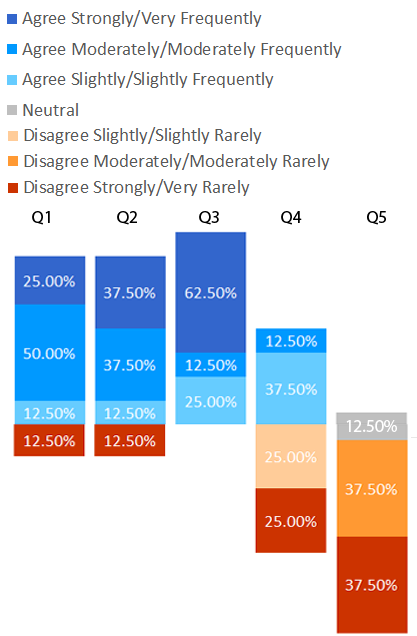
\includegraphics[width=0.9\marginparwidth]{lr2}
    \caption{Results for the 7-point Likert Scale Questionnaire}
    \label{fig:results}
\end{marginfigure}

\bibliography{sample-bibliography-sigchi-a}
\bibliographystyle{ACM-Reference-Format}

\end{document}